\subsection{Approach}

Coming up with the idea of the application and its functions has led to the realization that implementing a prototype with all the previously mentioned characteristics would lead to the prototype being dead on arrival, meaning that by the time it would be released it would most likely be already outdated. To counter this issue, startups and entrepreneurs often use an MVP approach for implementing the first prototype. 

The concept of MVP (Minimum Viable Product) is becoming increasingly important in the rapidly changing and evolving world of technology. The basis of this approach is that when developing a new product or service,  create  the simplest, yet most effective version to bring to market. 

There are several reasons to choose the MVP approach.
Rapid feedback and iteration means that when developers and entrepreneurs build a basic version of a product, they can quickly release it to users. Users can  share their thoughts and opinions about the product. This feedback is very important because it helps developers identify what changes and improvements need to be made to the product based on the actual wants and needs of users. Risk mitigation means doing things in a way that reduces the likelihood of problems occurring. 
 
An MVP strategy is to start with a simpler version of something and improve it  over time. This is helpful because it's easier and faster to create a simpler version, and then  developers can listen to people's opinions and improve it further. The methodology allows developers to focus on the most important parts of the product. This means you don't waste time creating things you don't need right away. If a product is really good and a lot of people like it, it's easier for manufacturers to get more funding to make it even better. That's because when you spend money making something, you find that many people want to use it and think it's a good idea. 
 
The main goal with this approach is for your product to reach the market faster. This is very important if other companies want to sell similar things, and if we are fast we can succeed. The MVP approach helps companies change quickly as needed. It also allows you to use your resources wisely and avoid wasting time and money on things that may not work. This is especially important in the world of technology, where things are always changing and people's needs are always changing. \cite{mvp}

\newpage

\subsection{Risk Management}

Without properly acknowledging the risks related to future of the development and production, it would not be sensible going forward with the software design. The table \ref{tab:risk} is responsible for showcasing the possible risks that are needed to be taken into account.

\begin{table}[ht]
	\centering
	\begin{tabularx}{\textwidth}{|l|X|}
		\hline
		\textbf{Risk Category} & \textbf{Risk Factors} \\ 
		\hline
		Technical Risks & Dependency on external APIs and web scraping for real-time data as well as for bar-code related data, challenges in ensuring cross-platform compatibility, potential scalability issues in handling large datasets. \\ 
		\hline
		Security Risks & Risks of data breaches or leaks, especially sensitive user data and scraped pricing information, security vulnerabilities regarding the API which could lead to loss of data and even legal issues. \\ 
		\hline
		Legal and Compliance Risks & Compliance with data protection laws (for example GDPR) when it comes to handling user data, legal issues related to web scraping and intellectual property rights, potential disagreements with supermarkets or other data sources. \\ 
		\hline
		Market and Business Risks & Dependence on supermarket partnerships, competition from already established and recognized price comparison and bar-code scanning applications, market acceptance and user adoption challenges, reliance on accurate and up-to-date pricing data. \\ 
		\hline
		Operational Risks & Challenges in maintaining and updating the application across different platforms, potential downtime or performance issues, managing a diverse technology stack with different characteristics. \\
		\hline
	\end{tabularx}
	\caption{Risk Management Analysis}
	\label{tab:risk}
\end{table}
\space

\subsection{Software Structure}

The solution is going to integrate a cloud-based database that can be accessed through a dedicated intermediate API. This API will also handle authorization, authentication and web scraping tasks.
This architecture is key to managing data flexibly and securely, ensuring high availability and scalability.

\newpage

The two main use cases of the solution are a mobile application for general users (iOS and Android) and a website that supports administrative tasks. All of these applications are based on the endpoints of the API for working with the data. The planned structure of the application can be visualized with figure \ref{fig:ur5}.
\begin{figure}[H]
	\centering
	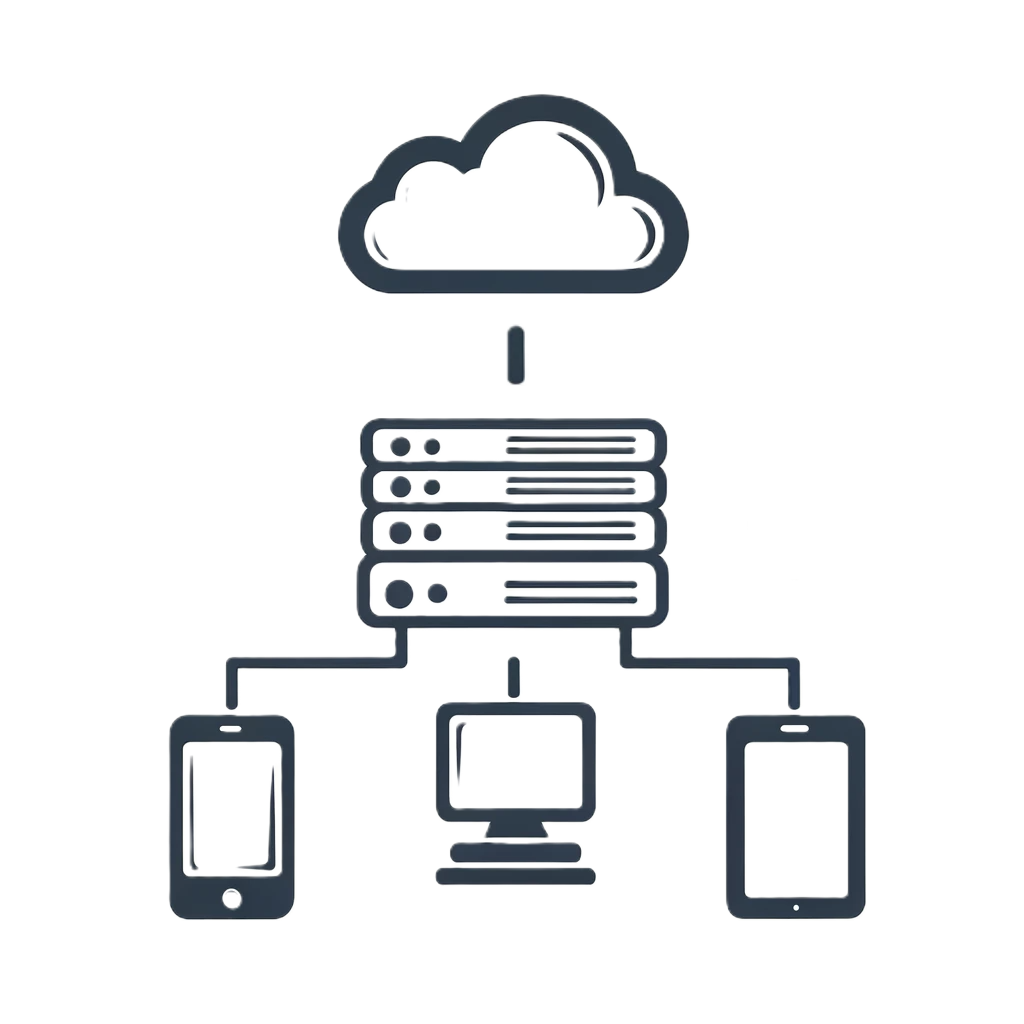
\includegraphics[width=0.5\linewidth]{img/architecturePlan.png}
	\caption{Visual Architecture Plan}
	\label{fig:ur5}
\end{figure}

This software architecture aligns well with the MVP approach to development and offers several benefits, such as:

\begin{itemize}
	\item \textbf{Security and privacy:} Planned cloud-based databases and intermediary APIs prioritize privacy. Advanced security protocols and encryption techniques are used to protect data stored in the cloud. Additionally, APIs that act as middle tiers provide additional protection when applications access databases through the middle tier.
	
	\item \textbf{Scalability and flexibility:} By deploying a cloud-based solution according to the  plan, you can easily adapt to the changing needs of your users.
	Additionally,  intermediate APIs allow applications running on different platforms to use the same data, eliminating the need to maintain separate databases for each platform.
	
	\item \textbf{Development efficiency:} By implementing standard data connections via the  API,  developers no longer need to create proprietary solutions for each platform.
	This significantly reduces development time and improves overall workflow efficiency.
	
	\item \textbf{Convenient maintenance and updates:} The Intermediate API allows the developer to centrally manage system maintenance and updates. This makes the application update process faster and more efficient.
	
	\item \textbf{Improved user experience:} Accessing cloud databases provides faster data processing and availability, which improves the user experience, especially when working with large amounts of data.
\end{itemize}
 
In summary, the proposed architecture aims to achieve a harmonious combination of security, scalability, development efficiency, and user experience while providing additional opportunities for application development. The solution shall provide users and administrators with modern, reliable, and efficient services at the same time.

\subsection{User Interface}

User-friendly design is the key to a successful mobile app. It helps with attracting and retaining users by providing an intuitive and user-friendly interface that increases user engagement and encourages them to spend more time with the app. Additionally, a well-designed app can improve brand image and encourage user loyalty. It can also contribute to reducing the need for frequent redesigns and upgrades, saving long-term development and maintenance costs, making it cost-effective. 

Understanding the needs and preferences of the target audience through user research and usability testing is the key to user-friendly design. The design needs to be clear and easy to navigate. Consistency in design elements improves usability and ensures a professional appearance. The design should also adapt to different devices and screen sizes to provide a consistent user experience. Additionally,  accessible design allows for a wider user base and enables social responsibility. \cite{userFriendly}

\begin{figure}[H]
	\centering
	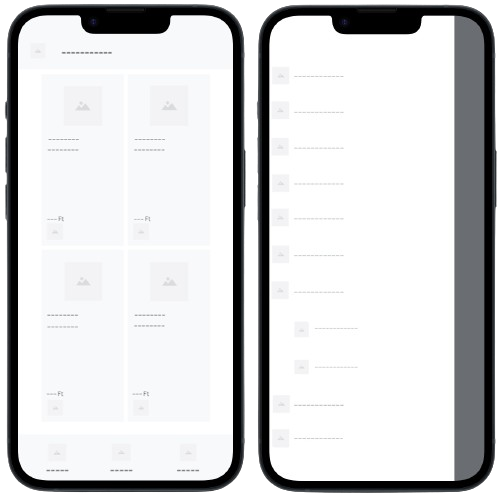
\includegraphics[width=0.3\linewidth]{img/ui_mockup.png}
	\caption{Mobile User Interface Mock-up}
	\label{fig:ur5}
\end{figure}

\subsection{Technological Stack}

The final product's overall success is largely dependent on the technological choices made during the project. A modern, flexible, and extremely efficient application can be developed by selecting a technology stack that includes MongoDB, ASP.NET, Angular, and .NET MAUI. When these technologies are combined, they form a strong and stable foundation that significantly raises the chances of project success. Each technology has advantages of its own.

\textbf{MongoDB} is a highly flexible and scalable data management system created especially for contemporary web applications is called {MongoDB}. Because it is a NoSQL database, it excels at managing dynamic data requirements, which makes it a great option for companies that operate in the fast-paced digital world of today. MongoDB manages enormous volumes of data with ease and is able to quickly adjust to changing data schemas thanks to its document-oriented architecture. Because of its remarkable flexibility, businesses can easily adapt their data models to the demands of their industries and quickly change their business requirements. Furthermore, the database can readily expand as the project grows thanks to MongoDB's built-in scalability and cloud-based deployment features, guaranteeing seamless performance and ideal data storage.

\textbf{ASP.NET API} is a powerful, incredibly secure framework with outstanding performance, which makes it a great option for creating enterprise applications. Developers can quickly and simply construct a dependable, orderly backend system that effectively manages a variety of client-side requests by using the ASP.NET API. Modern web applications can be built with the framework because of its built-in security features, which include support for RESTful APIs, optimization capabilities, and authentication and authorization.

\textbf{Angular} is a popular JavaScript framework created especially for making dynamic and interactive web applications. This adaptable framework gives developers a strong tool to quickly and effectively create user-friendly and responsive interfaces. It is made to function flawlessly across many platforms. With Angular's extensive feature set, which includes data binding, modular development, and testing capabilities, you can create beautiful, user-friendly websites that are both aesthetically pleasing and easy to maintain.

With the release of \textbf{.NET MAUI} by Microsoft, a cutting-edge framework created especially for cross-platform mobile application development is introduced. Using a single code base, developers can create top-notch apps for Windows, iOS, and Android platforms with this state-of-the-art framework. Developers can leverage the same code across platforms with.NET MAUI, saving a lot of money and time while still taking advantage of the distinct features and interfaces offered by each native operating system.


